
\chapter{Payload}
\label{chap:payload}

Without a Payload, there is no mission. The payload itself is significant for the design and layout of a rover system. It gives meaning and purpose to the system. The components of the payload carried along are examined in detail below. 

\section{Ground RADAR}
The Ground Radars main task is the identification of suitable drilling sites. Additionally, every radar campaign will contribute to further understanding of the ground composition on Europa.

Due to its small dimensions, the CRUX GPR is selected. The system is tested for lunar application at 800~MHz, resulting in a resolution of 15~cm and a penetration depth of 5~m \cite{CRUX_GPR}. The INSPIRE mission makes use of a 1.5~GHz frequency to increase the resolution. 
Reduced penetration depths are acceptable since the depth of interest for the ice core sampling is 10~cm (see \autoref{sec:IceCoreDrill}).

Additionally, high frequencies lead to a compact antenna design which is beneficial to the INSPIRE mission due to weight constraints. 
A custom patch antenna with the properties in \autoref{tab:GPR-A-Prp} is proposed \cite{patch_ant_GPR, Patch_Ant_design}.

\begin{table}[h]
\centering
\caption{GPR antenna properties \cite{Patch_Ant_design}.}
\begin{tabular}{lllll}
\toprule
Substrate ${\varepsilon}_\text{r}$ & Width & Length & Height & Mass   \\
\midrule
20                         & 30 mm & 20 mm  & 2 mm   & 2.73 g  \\
\bottomrule
\end{tabular}
\label{tab:GPR-A-Prp}
\end{table}

\section{Ice Core Drill} \label{sec:IceCoreDrill}
The Ice Core Drill is an in-house development based on drills from Honeybee Robotics \cite{Honeybee1, Honeybee2} and the drill from Philae \cite{PhilaeDrill}. The drill bit is made out of titanium to ensure that it does not deform or even breakthrough during the drilling process.
The ice core sample that can be obtained has a length of 100~mm and a diameter of 10~mm.
In order to save space, the drill is retracted while driving and will be extended for drilling, which is illustrated in the following \autoref{fig:DrillBay}.
After finishing the drill process, the drill retracts and the sample can be pushed out with the help of a piston, and meanwhile, it can be analysed by the APXS sensor.
When the sample has left the drill body, and the analysis is completed, the rover can switch back to locomotion mode and look for a new place to drill. As soon as a new drilling process starts, the previously taken sample falls to the ground to make room for a new one.

\begin{figure}[htb]
     \centering
     \begin{subfigure}[b]{0.45\textwidth}
         \centering
         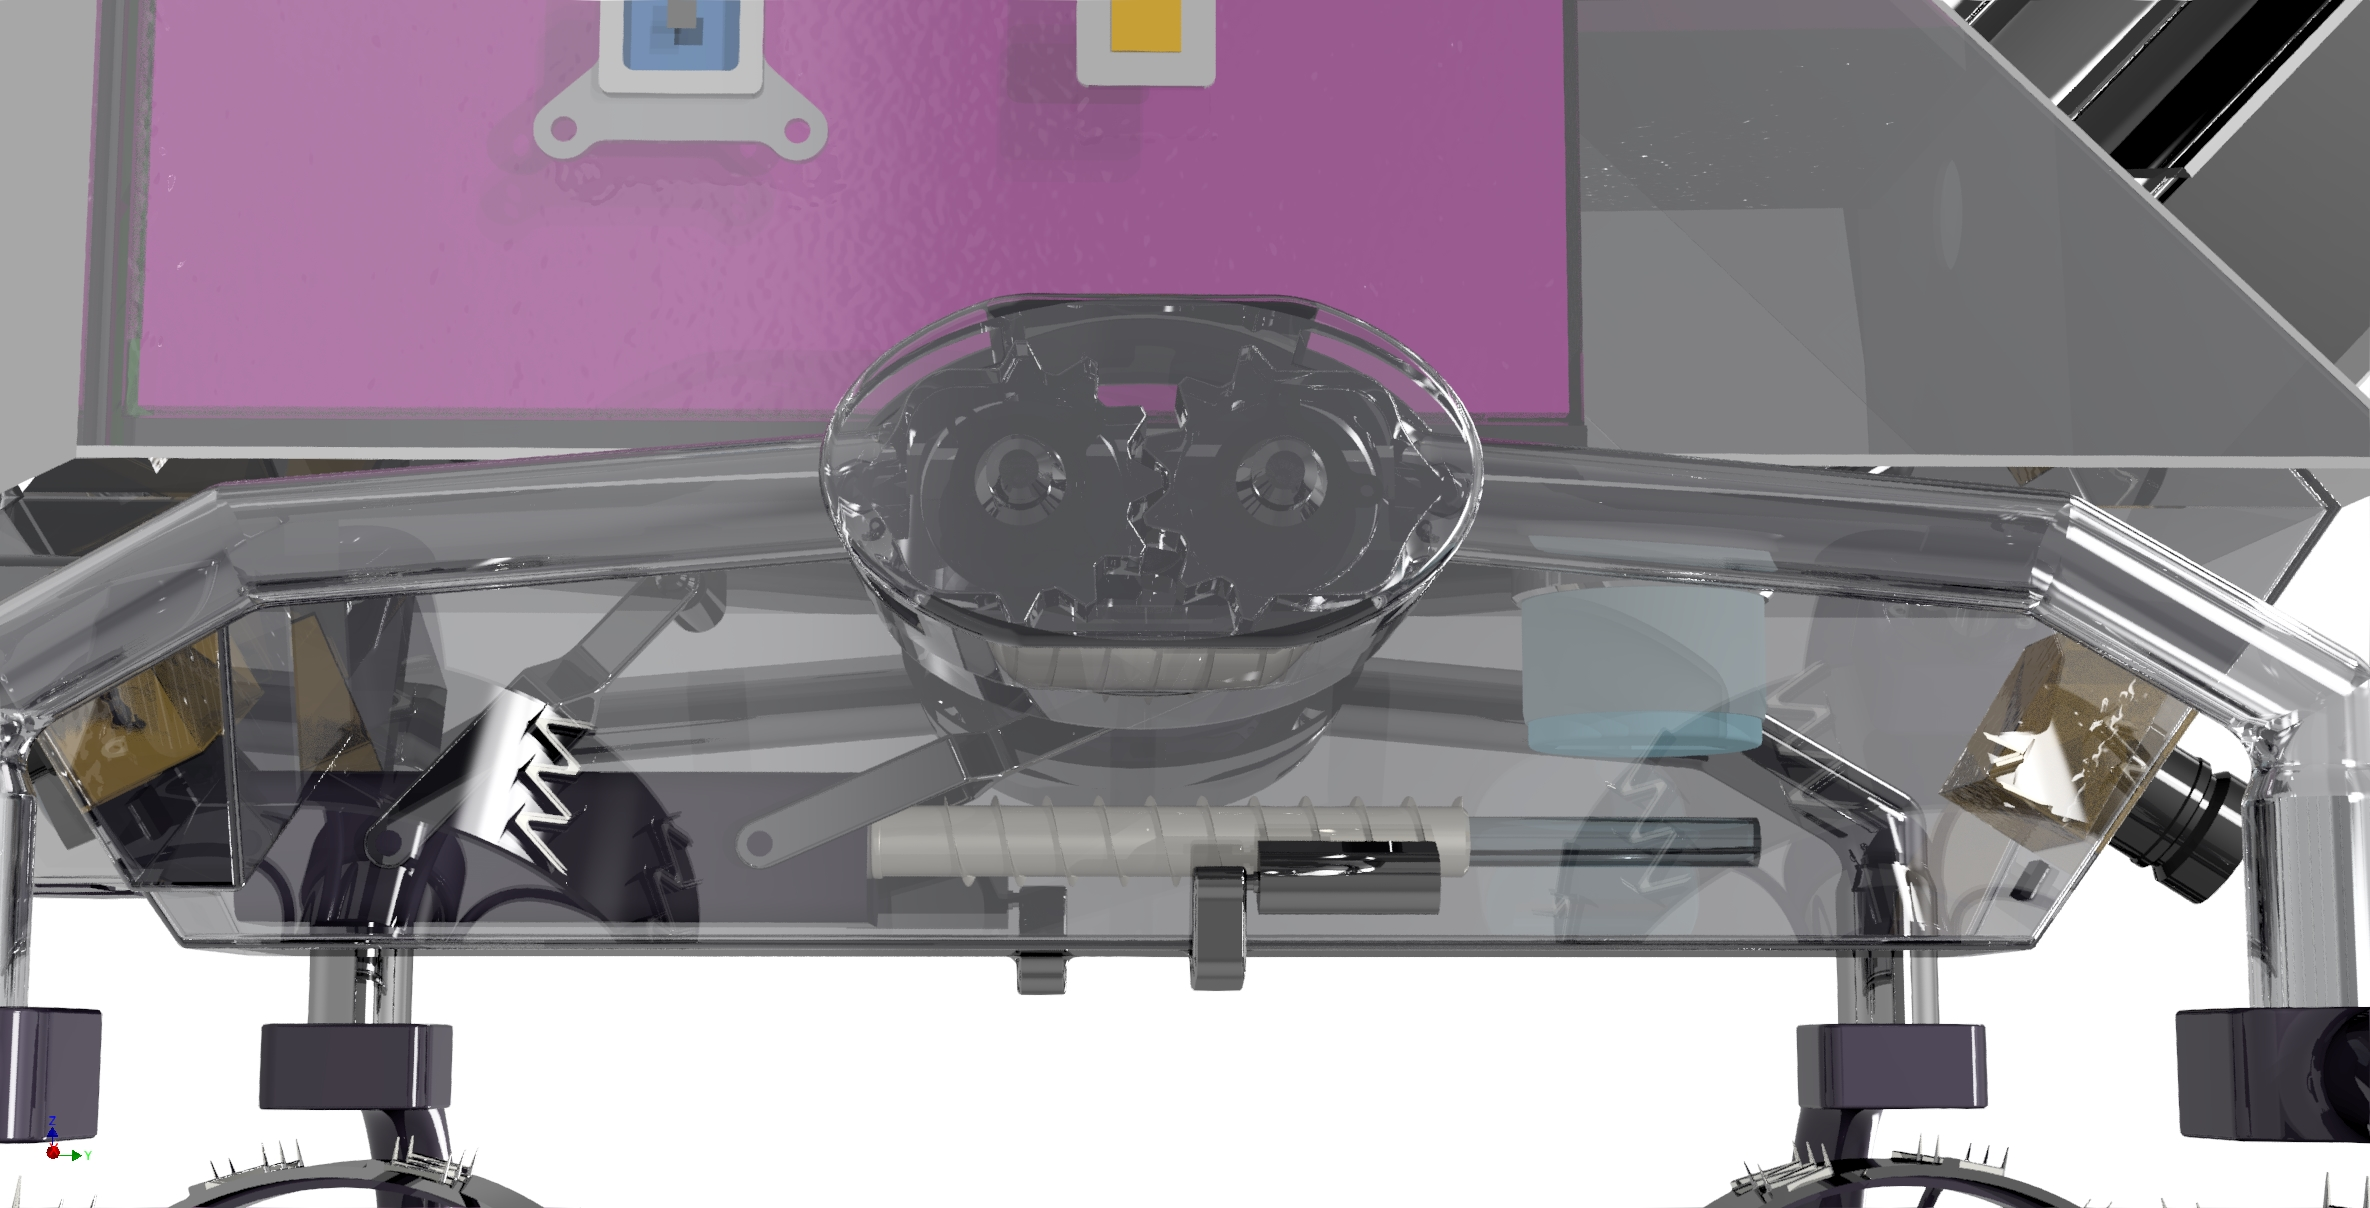
\includegraphics[width=\textwidth]{Media/DrillingBay3}
         \label{fig:stowedDrill}
     \end{subfigure}
     \hfill
     \begin{subfigure}[b]{0.45\textwidth}
         \centering
         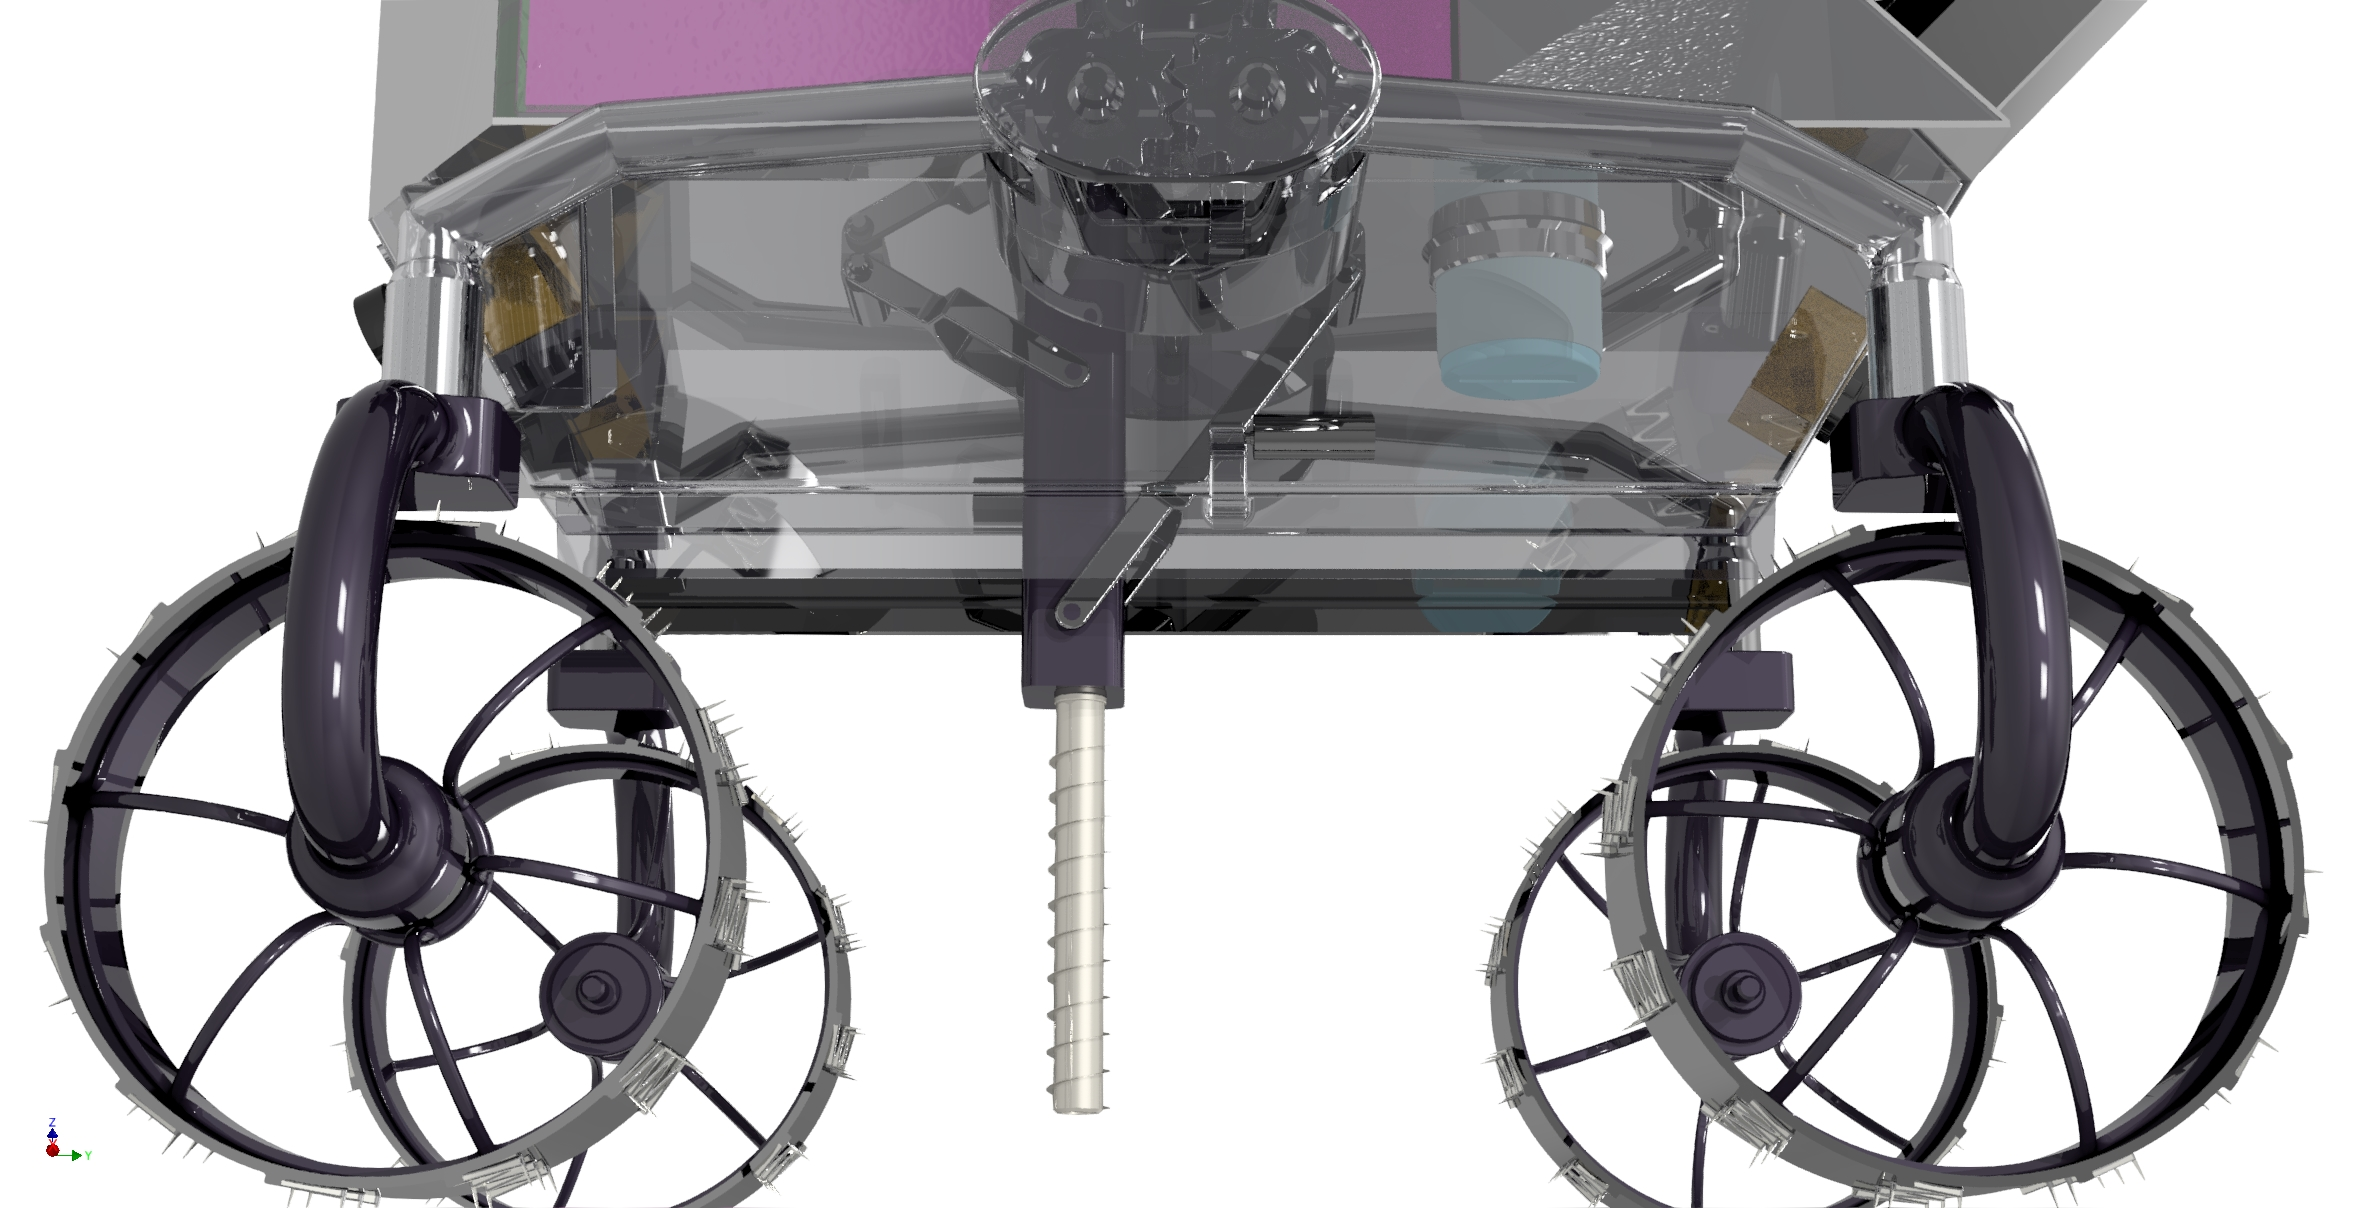
\includegraphics[width=\textwidth]{Media/DrillingBay_unfolded2}
         \label{fig:drillconfig}
     \end{subfigure}
     \hfill
     \caption{Left: Ice Core Drill in stowed configuration, Right: Ice Core Drill in drilling configuration}
     \label{fig:DrillBay}
\end{figure}

\section{APXS Analyser}
The Alpha Particle X-Ray Spectrometer is an analyser that has been used in many explorer missions like the Philae lander or the Mars rover Curiosity \cite{ref_pay_1, ref_pay_2}.
The spectrometer uses alpha particles as well as X-rays to identify the sort of atom inside a probe.
The main advantage is the small mass and the  low power it needs during the operation.
As a result of the relatively thin ice core samples, one-third of APXS sources and detectors will used.
Therefore, the mass and power consumption were downsized by one-third because the electronics keep the same and can't be reduced.


\section{Stereovision Camera / Observation / Perception}

The INSPIRE rover is equipped with five individual cameras. Two are used as stereo vision cameras on a hight-adjustable and rotatable telescope arm on the front side of the rover. This is used to capture a detailed 3D model of the environment with which sizes and distances can be estimated. The remaining three cameras are used as hazcams which are necessary to obtain data regarding the nearby environment. All cameras are equipped with radiation-hardened lenses to prevent browning of the lenses. Additional information is provided in \autoref{app:DigitalAppendix}. The main tasks of the camera system are the provision of scientific data and navigation-related data. %More details regarding the navigation and autonomy are provided in \autoref{sec:ControlandAutonomy}. \autoref{fig:CamHEad}

\begin{figure}[htb]
     \centering
     \begin{subfigure}[b]{0.45\textwidth}
         \centering
         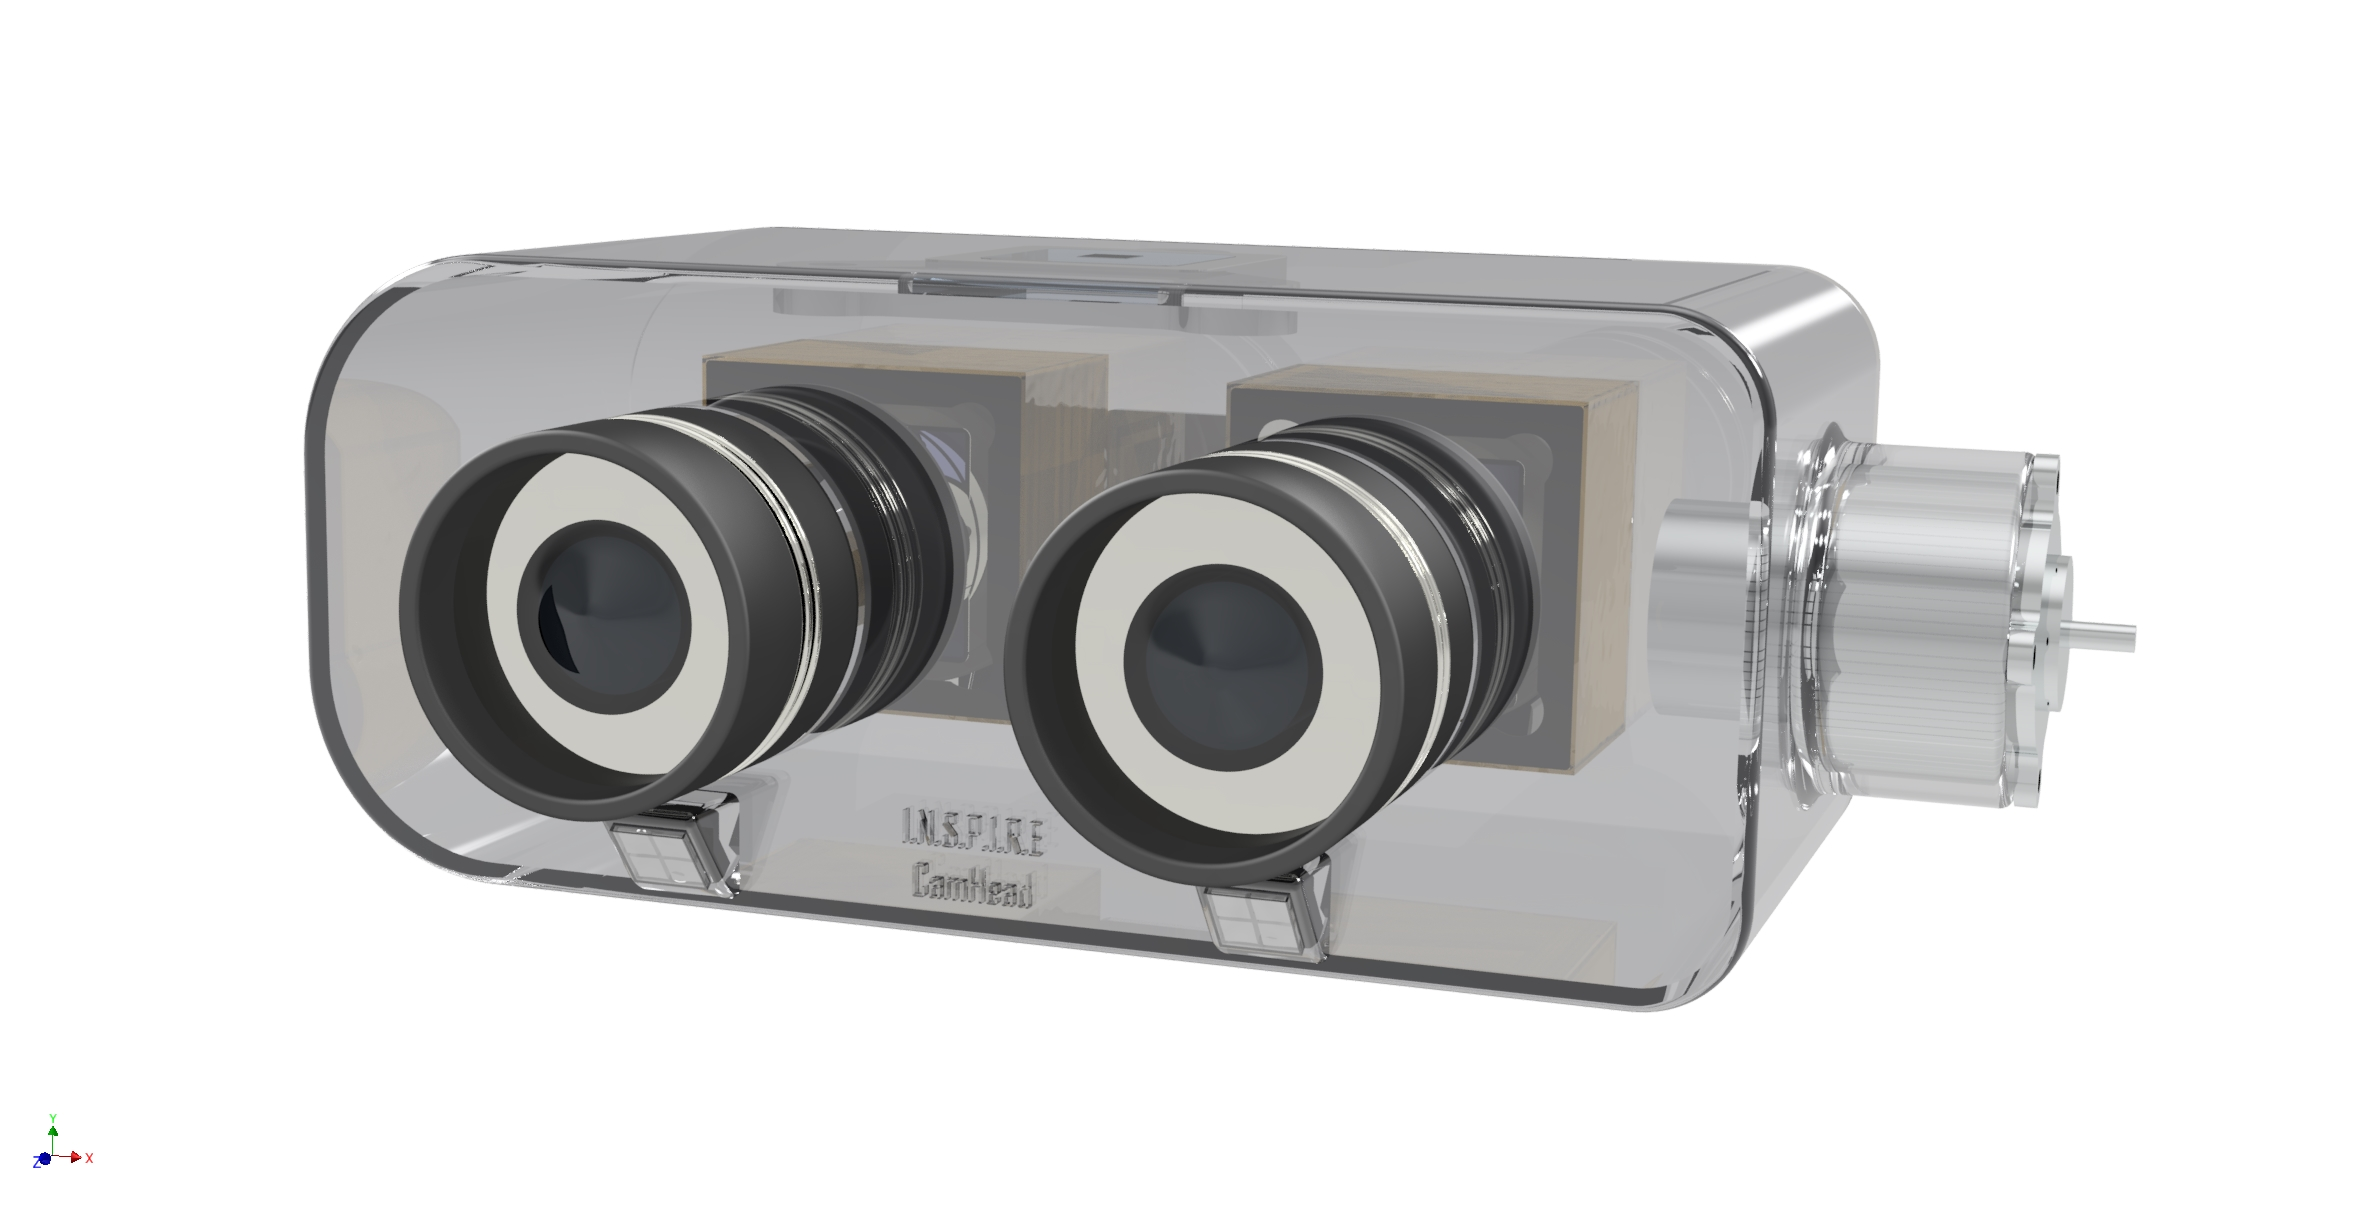
\includegraphics[width=\textwidth]{Media/CamHead}
         \label{fig:CamHead}
     \end{subfigure}
     \hfill
     \begin{subfigure}[b]{0.45\textwidth}
         \centering
         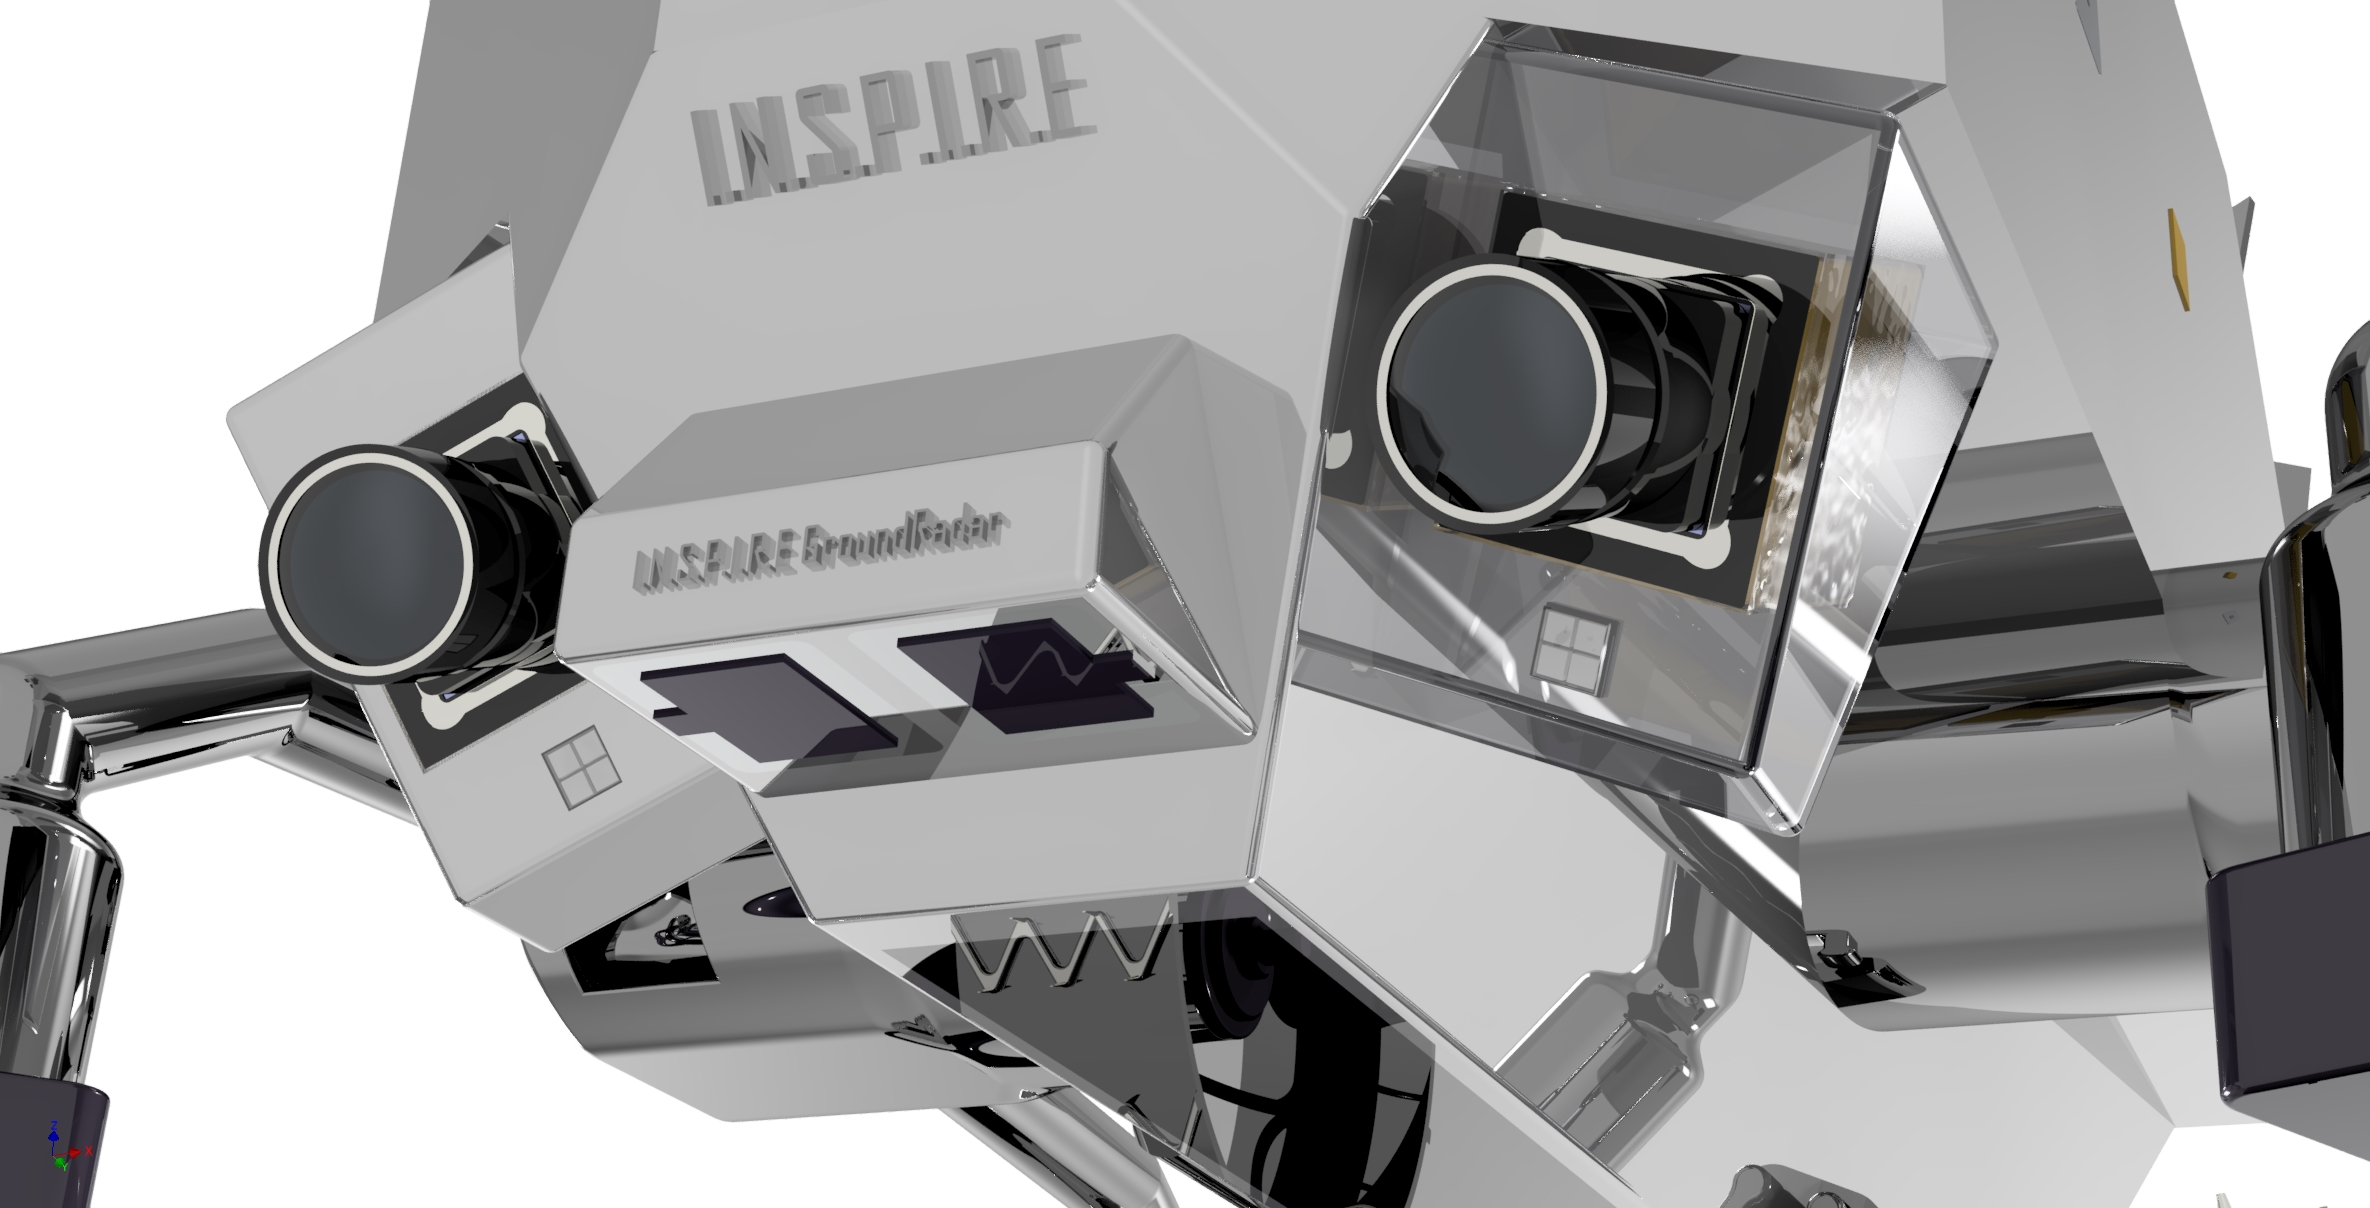
\includegraphics[width=\textwidth]{Media/HazCam_GroundRadar}
         \label{fig:HazCam}
     \end{subfigure}
     \hfill
     \caption{INSPIRE's Surface Observation System including CamHead and Hazcams + Ground Radar}
     \label{fig:Observation}
\end{figure}

\section{RadHard Solar Arrays}
\label{subsec:radhard}
As a secondary mission goal for INSPIRE, a cooperation with the European project RadHard, led by the German solar array manufacturer Azure Space is intended. The company currently develops a new generation of $4$ junction solar cells with up to $35~\% $ efficiency. However, the main feature of the new solar arrays is their radiation hardness which will be the highest radiation hardness of $>3~\% $ after $1E15~\text{cm}^{-2} \ 1~\text{MeV}$ electron irradiation. The Jupiter environment, with its extreme radiation, represents a suitable destination for a technology demonstration mission. Therefore INSPIRE will be equipped with $10$ RadHard solar cells with a total surface area of $0.0310~\text{m}^2$ as a technology demonstration \cite{FraunhoferInstituteforSolarEnergySystemsISE.2021}.

